
\ifdefined\ishandout
\documentclass[11pt,english,handout]{beamer}
\else
\documentclass[11pt,english]{beamer}
\fi

%\documentclass[11pt]{beamer}
\usepackage{mathptmx}
\renewcommand{\sfdefault}{lmss}
\renewcommand{\familydefault}{\sfdefault}
\usepackage[T1]{fontenc}
\usepackage[latin9]{inputenc}
\usepackage{amsmath}
\usepackage{amssymb}
\usepackage{graphicx}
\PassOptionsToPackage{normalem}{ulem}
\usepackage{ulem}
\usepackage{caption}
\captionsetup{labelformat=empty}
\usepackage{bbm}
\usepackage{upgreek}
\usepackage{graphicx}
\setbeamertemplate{section in toc}[sections numbered]
\makeatletter
\usepackage{caption} 
\usepackage{bm}
\usepackage{subfig}
\captionsetup[table]{skip=10pt}
%%%%%%%%%%%%%%%%%%%%%%%%%%%%%% Textclass specific LaTeX commands.
% this default might be overridden by plain title style
\newcommand\makebeamertitle{\frame{\maketitle}}%
% (ERT) argument for the TOC
\AtBeginDocument{%
	\let\origtableofcontents=\tableofcontents
	\def\tableofcontents{\@ifnextchar[{\origtableofcontents}{\gobbletableofcontents}}
	\def\gobbletableofcontents#1{\origtableofcontents}
}

%%%%%%%%%%%%%%%%%%%%%%%%%%%%%% User specified LaTeX commands.
%\documentclass[presentation]{beamer}


\def\Tiny{\fontsize{7pt}{8pt}\selectfont}
\def\Normal{\fontsize{8pt}{10pt}\selectfont}

\usetheme{Madrid}
\usecolortheme{lily}
%\setbeamercovered{transparent}
\useinnertheme{rounded}


\setbeamertemplate{footline}{\hfill\Normal{\insertframenumber/\inserttotalframenumber}}
%\setbeamertemplate{footline}{}

\setbeamertemplate{navigation symbols}{}

\newenvironment{changemargin}[2]{%
	\begin{list}{}{%
			\setlength{\topsep}{0pt}%
			\setlength{\leftmargin}{#1}%
			\setlength{\rightmargin}{#2}%
			\setlength{\listparindent}{\parindent}%
			\setlength{\itemindent}{\parindent}%
			\setlength{\parsep}{\parskip}% 
		}%
		\item[]}{\end{list}}

\setbeamertemplate{footline}{\hfill\insertframenumber/\inserttotalframenumber}
\setbeamertemplate{navigation symbols}{}

%\usepackage{times}  % fonts are up to you
\usepackage{graphicx}
%\usepackage{graphics}
\usepackage{epsfig}
\usepackage{bm}
\usepackage{epsf}
\usepackage{float}
\usepackage[final]{pdfpages}
\usepackage{multirow}
\usepackage{colortbl}
\usepackage{xkeyval}
%\usepackage{sgame}
%\usepackage{pst-node}
\usepackage{listings}
\usepackage{ifthen}
%\usepackage{hyperref}
\usepackage{tikz}

%\usepackage{times}  % fonts are up to you
%\usepackage{graphicx}
%\usepackage{graphics}
\usepackage{epsfig,bm,epsf,float}
\usepackage[final]{pdfpages}
\usepackage{xcolor,multirow,colortbl}
\usepackage{xkeyval}
\usepackage{verbatim}
%\usepackage{sgame}
%\usepackage{pst-node}
\usepackage{listings}
%\usepackage{handoutWithNotes}
%\pgfpagesuselayout{3 on 1 with notes}[letterpaper,border shrink=5mm]
%\pgfpagesuselayout{2 on 1 with notes landscape}[letterpaper,border shrink=5mm]
\usepackage{setspace}
\usepackage{ragged2e}

\setbeamersize{text margin left=1em,text margin right=1em} % CambridgeUS spacing if you use default instead


%\pdfmapfile{+sansmathaccent.map}

% Table formatting
\usepackage{booktabs}


% Decimal align
\usepackage{dcolumn}
\newcolumntype{d}[0]{D{.}{.}{5}}


\global\long\def\expec#1{\mathbb{E}\left[#1\right]}
\global\long\def\var#1{\mathrm{Var}\left[#1\right]}
\global\long\def\cov#1{\mathrm{Cov}\left[#1\right]}
\global\long\def\prob#1{\mathrm{Prob}\left[#1\right]}
\global\long\def\one{\mathbf{1}}
\global\long\def\diag{\operatorname{diag}}
\global\long\def\expe#1#2{\mathbb{E}_{#1}\left[#2\right]}
\DeclareMathOperator*{\plim}{\text{plim}}

%\usefonttheme[onlymath]{serif}

\usepackage{appendixnumberbeamer}
\renewcommand{\thefootnote}{}

\setbeamertemplate{footline}
{
	\leavevmode%
	%   \hbox{%
	%      \begin{beamercolorbox}[wd=\paperwidth,ht=2.25ex,dp=1ex,right]{date in head/foot}%
	%\usebeamerfont{date in head/foot}\insertshortdate{}\hspace*{2em}%
	\hfill
	%turning the next line into a comment, erases the frame numbers
	\insertframenumber{}\hspace*{2ex}\vspace{1ex}
	
	%    \end{beamercolorbox}}%
}

\definecolor{blue}{RGB}{0, 0, 210}
\definecolor{red}{RGB}{170, 0, 0}

\makeatother

\usepackage[english]{babel}

\usepackage{tikz}
\newcommand*\circled[1]{\tikz[baseline=(char.base)]{             \node[circle,ball color=structure.fg, shade,   color=white,inner sep=1.2pt] (char) {\tiny #1};}} 

\makeatletter
\let\save@measuring@true\measuring@true
\def\measuring@true{%
	\save@measuring@true
	\def\beamer@sortzero##1{\beamer@ifnextcharospec{\beamer@sortzeroread{##1}}{}}%
	\def\beamer@sortzeroread##1<##2>{}%
	\def\beamer@finalnospec{}%
}
\makeatother



\setbeamersize{text margin left= .8em,text margin right=1em} 
\newenvironment{wideitemize}{\itemize\addtolength{\itemsep}{10pt}}{\enditemize}
\newenvironment{wideitemizeshort}{\itemize}{\enditemize}

\newcommand{\indep}{\perp\!\!\!\!\perp} 


\DeclareMathOperator*{\argmax}{arg\,max}
\DeclareMathOperator*{\argmin}{arg\,min}

\begin{document}
	
	%% Title slide
	\begin{frame}[noframenumbering]{}
		\vspace{0.5cm}
		\title[]{Chapter 6: Panel Data}
		\author{Jonathan Roth}
		\date{Mathematical Econometrics I \\ Brown University\\ Fall 2023} 
		\titlepage {\small{}\ }\thispagestyle{empty} \vspace{-30pt}
		
	\end{frame}

	
	\begin{frame}{Motivation}
		
		\begin{wideitemize}
			\item
			We've seen how to estimate causal effects when a treatment is as good as randomly assigned conditional on observable characteristics
			
			\item
			But often we're worried that there are unobservable characteristics we haven't properly accounted for (i.e. confounding variables)
			
			\pause
			\item
			Next we'll think about how we can deal with certain types of unobserved confounding variables when we have \textbf{panel data}

			
		\end{wideitemize}

	\end{frame}

\begin{frame}{What is Panel Data?}
	\begin{wideitemize}
	\item
	Panel data refers to a situation where we observe observations for each unit $i$ (say a person or state) across multiple periods $t$				
	
	\pause
	\item
	Why is this useful? It allows us to look at differences in outcomes between treated/untreated units \textit{before} the treatment occurred
	
	\pause
	\item
	If treated/control outcomes are different before the treatment, this must be the result of confounding factors.
	
	\pause
	\item
	So we can potentially use pre-treatment differences to learn about the confounds and adjust for them
	
	\pause
	\item
	Let's see how this works in an example of \textbf{difference-in-differences}, which is the most common panel data method used in applied microeconomic research
	\end{wideitemize}

\end{frame}	



\begin{frame}{Hastings (2004)}
\begin{wideitemize}
	\item
	In 2004, Justine Hastings (a former Brown prof!) wrote a study analyzing how mergers in the gas industry affect gas prices 
	
	\pause
	\item
	In particular, she studied an episode in California where a refinery, ARCO, bought one of the largest gas stations, Thrifty
	
	\pause
	\item
	How do you think such a merger might affect prices? 
	\pause
		\begin{itemize}
			\item 
			On the one hand, it could reduce competition and increase prices
			\item
			On the other, a merger could reduce costs of providing gas and decrease prices (synergies)
		\end{itemize}

	
	\pause
	\item
	Hastings attempted to answer this question empirically using data on gas prices by neighborhood in CA 
		\begin{itemize}
			\item
			Data contains info on neighborhoods both with/without Thrifty stations 
		\end{itemize}	
	 
\end{wideitemize}
	
\end{frame}
	
	
\begin{frame}
	\begin{wideitemize}
		\item 
		Suppose first that we only had data on gas prices from after the merger occurred.
		
		\item
		We could compare prices in areas that had a Thrifty beforehand ($D_i = 1$) and places that didn't have a Thrifty beforehand ($D_i=0$) to estimate the causal effect of a Thrifty conversion
		
		\pause
		\item
		Why might this not give us the causal effect of converting Thrifties? \pause Omitted variables!
		
		\pause
		\item
		In particular, places that already had a Thrifty beforehand likely had more competition than places without a Thrifty. We thus might expect them to have lower prices.
		
		\pause
		\item
		With panel data, we can test this empirically by looking at prices before the merger!
	\end{wideitemize}
\end{frame}	


\begin{frame}
	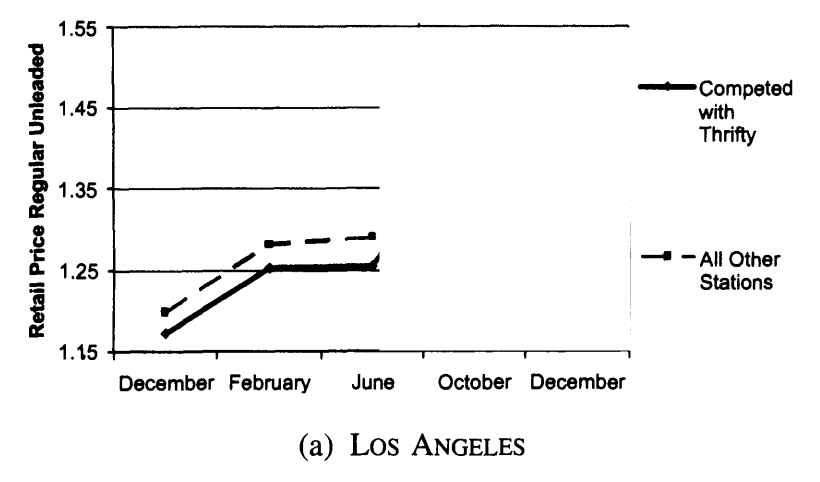
\includegraphics[width=0.7\linewidth]{hastings-event-study-pre}
	\begin{wideitemize}
		\item
		Before the merger, stations in markets competing with Thrifty had gas prices about 3 cents lower in every period
		
		\pause
		\item
		Is it reasonable to assume unconfoundedness after the merger? \pause No!
		
		\pause
		\item
		A better assumption might be that the gap would haved remained 3c if not for the merger! \pause{} This is the idea of \textbf{difference-in-differences}
	\end{wideitemize}
\end{frame}

\begin{frame}
	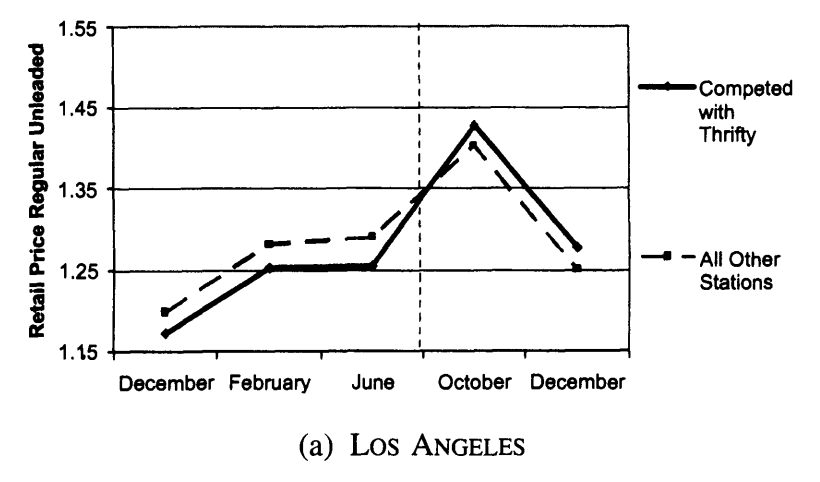
\includegraphics[width=0.7\linewidth]{hastings-event-study}

	\begin{wideitemize}
		\item
		After the merger, stations in areas with a Thrifty had \textit{higher prices} by about 2c
		
		\pause
		\item
		If we assume that they would have had \textit{lower} prices by 3c (as before the merger), then this implies a treatment effect of \pause{} $2 - (-3) = 5$ 
		
		\pause
		\item
		This is the post-treatment difference (2) between treatment \& control minus the pre-treatment difference (-3), i.e. a \textit{difference-in-differences}
	\end{wideitemize}

\end{frame}

\begin{frame}{Formalizing the Assumptions of DiD}
\begin{wideitemize}
	\item
	Assume there are 2 periods, $t = 1,2$.  Treated units ($D_i=1$) are treated in period 2; control units never-treated.
	
	\item
	Let $Y_{it}$ be the observed outcome for unit $i$ in period $t$. \\ 
	Assume $Y_{it} = D_{i} Y_{it}(1) + (1-D_i)Y_{it}(0)$
	
	\pause
	\item
	\textbf{No anticipation assumption}: $Y_{i1}(0) = Y_{i1}(1)$
		\begin{itemize}
			\item 
			Your treatment in period 2 doesn't affect your outcome in period 1
		\end{itemize}	
	\item
	\textbf{Parallel trends assumption}:
	$$ \underbrace{E[  Y_{i2}(0) - Y_{i1}(0) | D_i = 1 ] }_{\text{Change in $Y(0)$ for treated}} = \underbrace{E[  Y_{i2}(0) - Y_{i1}(0) | D_i = 0 ] }_{\text{Change in $Y(0)$ for control}} $$
	
	\pause
	Equivalently,
	$$\scriptsize \underbrace{E[  Y_{i2}(0) | D_i = 1 ] - E[Y_{i2}(0) | D_i =0] }_{\text{Selection bias in period 2}} = \underbrace{E[  Y_{i1}(0) | D_i = 1 ] - E[Y_{i1}(0) | D_i =0] }_{\text{Selection bias in period 1}} $$
\end{wideitemize}	
\end{frame}

\begin{frame}
\begin{wideitemize}
	\item 
	Under these assumptions, we have
	\begin{align*}
	& \underbrace{E[Y_{i2} - Y_{i1} | D_i = 1 ]}_{\text{Observed change for treated}} - \underbrace{E[Y_{i2} - Y_{i1} | D_i = 0 ]}_{\text{Observed change for control}} = \\
	&= E[Y_{i2}(1) - Y_{i1}(1) | D_i = 1 ] - E[Y_{i2}(0) - Y_{i1}(0) | D_i = 0 ] \text{ \scriptsize (Observed data rule) } \pause{}\\
	&= E[Y_{i2}(1) - Y_{i1}(0) | D_i = 1 ] - E[Y_{i2}(0) - Y_{i1}(0) | D_i = 0 ] \text{ \scriptsize (No anticipation) } \pause{} \\
	&  = E[Y_{i2}(1) - Y_{i2}(0) | D_i = 1] + \\&  E[Y_{i2}(0) - Y_{i1}(0) | D_i = 1 ] - E[Y_{i2}(0) - Y_{i1}(0) | D_i = 0 ]  \text{\scriptsize  (Adding and subtracting) } \pause{}\\
	&= E[Y_{i2}(1) - Y_{i2}(0) | D_i = 1] \text{ \scriptsize(Parallel trends) }
	\end{align*}

	\pause
	\item
	Thus, the difference-in-difference of sample means identifies $\tau_{ATT} = E[Y_{i2}(1)- Y_{i2}(0) | D_i = 1]$.
	
	\item
	This is called the \textbf{average treatment effect on the treated} (ATT).\\
	It is the average effect in period 2 for treated units.
	
\end{wideitemize}
\end{frame}
	
	
\begin{frame}{Estimating the ATT}
	\begin{wideitemize}
		\item
		We've shown that under the DiD assumptions (parallel trends and no anticipation), the ATT is identified as
		$$ \tau_{ATT} = \underbrace{E[Y_{i2} - Y_{i1} | D_i = 1 ]}_{\text{Change in pop mean for treated}} - \underbrace{E[Y_{i2} - Y_{i1} | D_i = 0 ]}_{\text{Change in pop mean for control}}  $$
		
		\item
		How can we estimate this? \pause{} Plug in sample means!
		
		\pause
		\item
		Our estimate is: 
		$$\hat\tau_{ATT} = \underbrace{\bar{Y}_{12} - \bar{Y}_{11} }_{\text{Change in sample mean for treated}} - \underbrace{\bar{Y}_{02} - \bar{Y}_{01}}_{\text{Change in sample mean for control}} , $$
		
		\noindent where $\bar{Y}_{dt}$ is the sample mean for units with $D_i =d $ in period $t$. 
		
	\end{wideitemize}
\end{frame}	

\begin{frame}{Example}
	\begin{itemize}
		\item 
		Consider Hasting's example, comparing June (period 1) to October
	\end{itemize}
	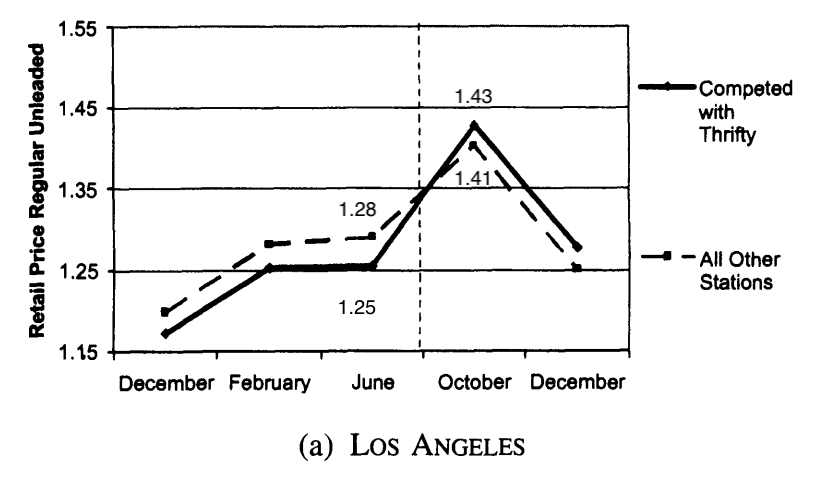
\includegraphics[width =.7\linewidth]{hastings-event-study-w-labels}

\pause
		\begin{align*}
			\hat\tau_{ATT}=&  \underbrace{\bar{Y}_{12} - \bar{Y}_{11} }_{\text{Change in sample mean for treated}} - \underbrace{\bar{Y}_{02} - \bar{Y}_{01}}_{\text{Change in pop mean for control}} =\\& \pause{} (1.43 - 1.25) - (1.41 - 1.28) = \pause{} 0.05
		\end{align*} 

\end{frame}



\begin{frame}{DiD as Regression}
	\begin{itemize}
		\item 
		Consider the regression 
		$$Y_{it} = \beta_0 + \beta_1 \times Post_t + \beta_2 D_i + \beta_3 D_i \times Post_t + \epsilon_{it},$$
		\noindent where $Post_t = 1[t=2]$.
		
		\pause
		\item
		Claim: the population regression coefficient $\beta_3$ is equal to $\tau_{ATT}$ under the DiD assumptions.
		
		\pause
		\item
		Why? The regression above models the CEF as:
		\begin{align*}
			& E[Y_{it} | D_i = 0, Post_t = 0 ]  = \pause{}  \beta_0 \pause{} \\
			& E[Y_{it} | D_i = 0, Post_t = 1 ] = \pause{}  \beta_0 + \beta_1 \pause{} \\ 
			& E[Y_{it} | D_i = 1, Post_t = 0 ] = \pause{}  \beta_0 + \beta_2 \pause{} \\
			& E[Y_{it} | D_i = 1, Post_t = 1 ] = \pause{}  \beta_0 + \beta_1 + \beta_2 + \beta_3
		\end{align*}
	
	\pause
	\item
	Thus, 
	\begin{align*}
	\beta_3 = &(E[Y_{it} | D_i = 1, Post_t = 1 ] - E[Y_{it} | D_i = 1, Post_t = 0 ]) - \\ &(E[Y_{it} | D_i = 0, Post_t = 1 ] - E[Y_{it} | D_i = 0, Post_t = 0 ]) = \tau_{ATT}		
	\end{align*}

\pause
\item Analogously, $\hat\beta_3 = (\bar{Y}_{12} -\bar{Y}_{11}) - (\bar{Y}_{02} -\bar{Y}_{01}) = \hat\tau_{ATT}$

	\end{itemize}
\end{frame}

\begin{frame}{Example}

\begin{center}
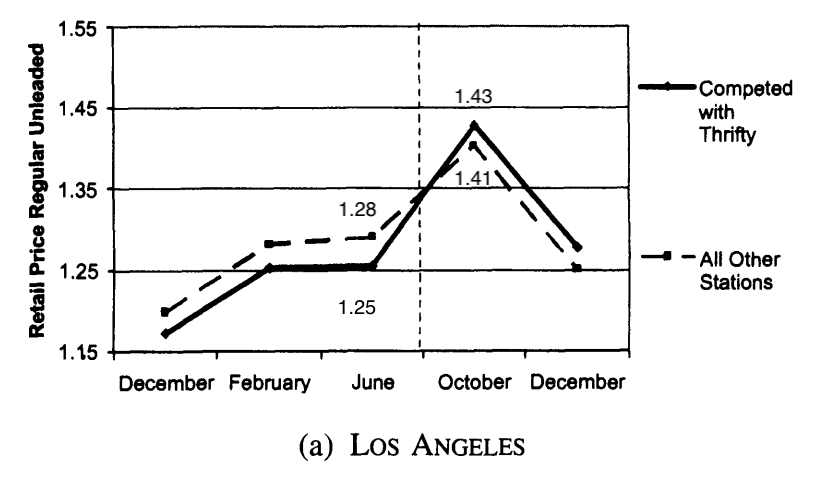
\includegraphics[width = 0.5\linewidth]{hastings-event-study-w-labels}
\end{center}
\begin{wideitemize}


\item
Suppose we take the Hastings data from June/October and estimate
$$Y_{it} = \beta_0 + \beta_1 \times Post_t + \beta_2 D_i + \beta_3 D_i \times Post_t + \epsilon_{it},$$
\noindent via OLS, where $Post_t$ is 1 for October and 0 for June. 

\pause
\item
We get the regression coefficients:
\begin{tabular}{lr}
Constant ($\hat\beta_0$) & 1.28 \\
Post ($\hat\beta_1$) & 0.13 \\
Treated ($\hat\beta_2$) & -0.03 \\
Treated $\times$ Post ($\hat\beta_3$) & 0.05
\end{tabular}
\end{wideitemize}	
\end{frame}


\begin{frame}{DiD with Multiple Periods}
	
	\begin{wideitemize}
		\item
		Often we have more that 2 periods for a DiD analysis\pause{}
		
		\item
		This is useful for two reasons: \pause{}
		
		\begin{enumerate}
			\item 
			We can test whether parallel trends appears to hold \textit{prior} to treatment\pause{}
			
			\pause
			\item
			We can analyze how the ATT changes over time \pause{}
		\end{enumerate}


		\item
		How do we do this? 

	\end{wideitemize}
\end{frame}


\begin{frame}{DiD with Multiple periods}
	\begin{wideitemize}
		\item
		Suppose that we have periods $t=-\underline{T},...,\bar{T}$. Treated units begin getting treatment at period 1.
		
		\pause
		\item
		For each period $s \neq 0$, we can estimate a 2-period DiD between period $s$ and period 0:
		
		$$\hat\beta_s = \underbrace{(\bar{Y}_{1s} - \bar{Y}_{0s})}_{\text{Diff in period $s$}} -  \underbrace{(\bar{Y}_{10} - \bar{Y}_{00})}_{\text{Diff in period 0}} $$
		
		\noindent where $\bar{Y}_{dt}$ is the average for treatment group $d$ in period $t$.
		
		\pause
		\item
		Conveniently, the $\hat\beta_s$ are equal to the OLS estimates of the regression
		
		$$Y_{it} =  \phi_{t} + D_i \gamma + \sum_{s\neq 0}  D_i \times 1[t = s] \times  \beta_s   + \epsilon_{it} $$
		
		\pause
		\item
		You can also replace $D_i \gamma$ with a unit fixed effect $\lambda_i$ and you get the exact same $\hat\beta_s$. 
		\end{wideitemize}
\end{frame}

\begin{frame}{Example - Medicaid Expansion}
	
	\begin{wideitemize}
		\item
		The Affordable Care Act (ACA, aka Obamacare) expanded Medicaid coverage to people with income up to 138\% of the federal poverty line
		
		\item
		Medicaid expansion went into effect in 2014. However, some Republican-leaning states opted out of expanded coverage.
		
		\item
		By 2015, 24 states had expanded Medicaid (more have done so since)
		
		\pause
		\item
		Carey, Miller, and Wherry (2020) study the impacts of Medicaid expansion using a DiD design comparing early-adopting states to non-adopters.
				
		
	\end{wideitemize}
	
\end{frame}

\begin{frame}{Example - Medicaid Expansion}
	\begin{wideitemize}
		\item
		A slightly simplified version of their regression specification is
		
		$$Y_{its} =  \phi_{t} + \lambda_s + \sum_{r\neq -1}  D_i \times 1[t = 2014 + r] \times  \beta_r   + \epsilon_{it} $$
		
		\noindent where $Y_{its}$ is outcome for person $i$ in year $t$ in state $s$, and $D_i = 1$ if in an expansion state.\pause{} Lets plot the $\beta_s$ estimates and 95\% CIs:
	\end{wideitemize}\pause{}
	
	
	\begin{center}
		\includegraphics[width = 0.6 \linewidth]{carey-event-study}
	\end{center}
	
	
	\pause
	\begin{itemize}
		\item
		Results show similar ``pre-trends'' but negative effects after treatment 
	\end{itemize}

\end{frame}


\begin{frame}
In a related paper, some of the same authors used a similar research design to estimate the impacts on mortality
\begin{center}
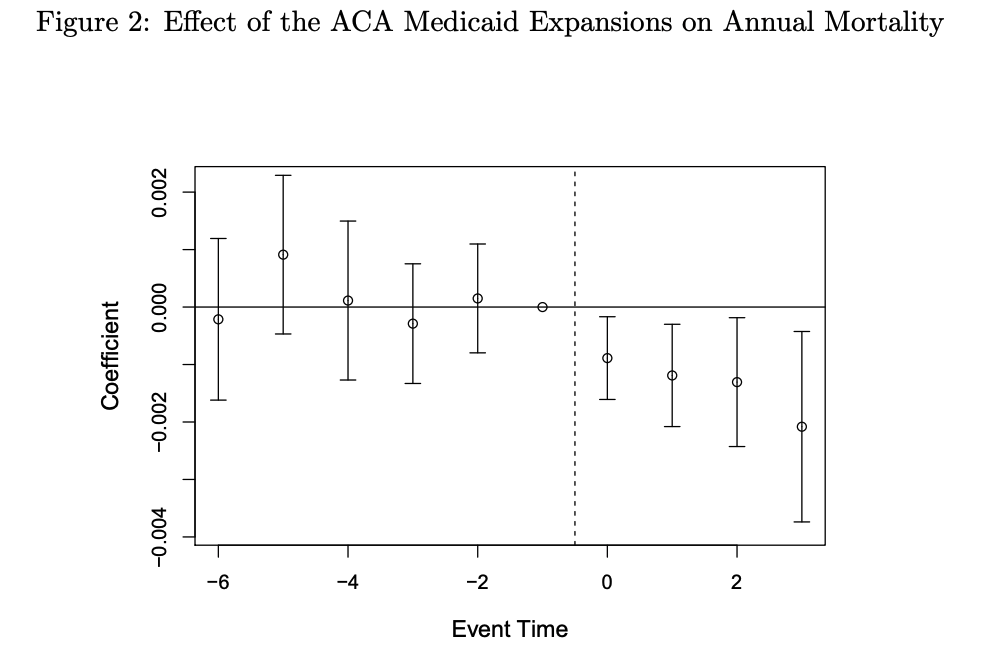
\includegraphics[width = 0.7\linewidth]{medicaid-mortality}
\end{center}
\end{frame}


\begin{frame}{Some Caution about Parallel Trends}
	
	\begin{wideitemize}
		\item
		DiD relies on the parallel trends assumption, which allows for selection bias but requires it to be stable over time. \pause This rules out time-varying confounding factors.
		
		\pause
		\item
		Often we will be worried about time-varying confounds --- e.g., macro-economic factors might differentially affect Democratic versus Republican states		 
		
		\pause
		\item
		Testing for pre-treatment differences (``pre-trends'') can help increase our confidence in the research design. \pause But they're not perfect. Why? 
		
		\begin{enumerate}
			\item 
			Just because trends were parallel beforehand doesn't mean that they would continue to be afterwards
			
			\pause
			\item
			Often our estimates of pre-trends are noisy so we're not sure whether they're actually zero or not.
		\end{enumerate}
	\end{wideitemize}

\end{frame}

\begin{frame}
\begin{wideitemize}
	\item
	In addition to looking at the point estimates of pre-trends, it's important to consider what the CIs rule out
	
	\pause
	\item
	A good rule of thumb for whether a plot is convincing is whether you can draw a smooth line through all the confidence intervals
\end{wideitemize}

\pause
\begin{onlyenv}<+>
\centering
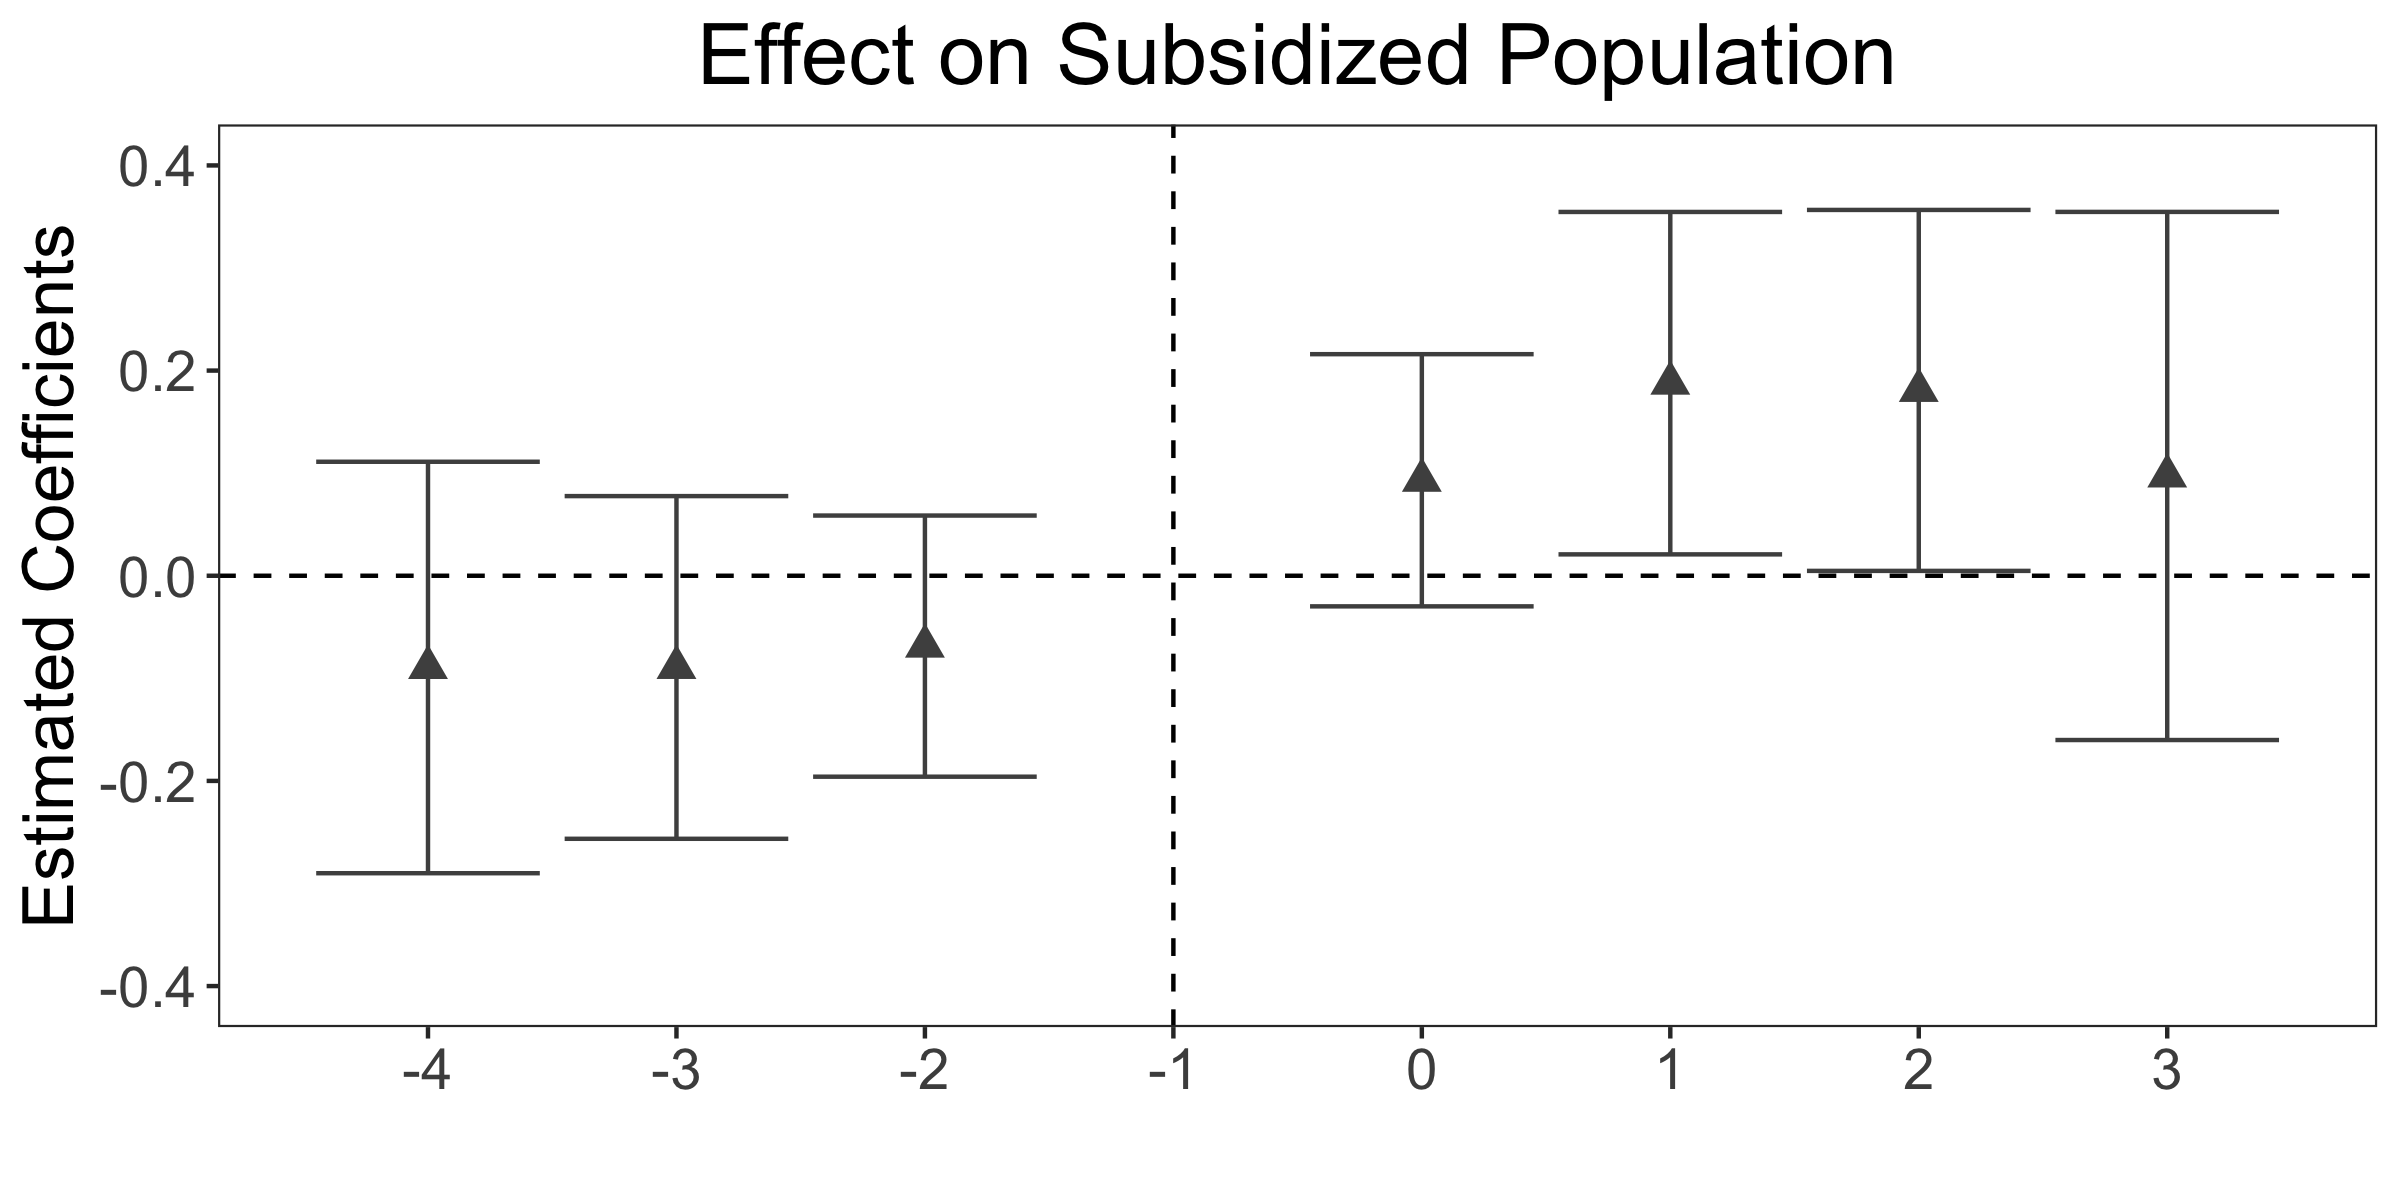
\includegraphics[width = 0.7 \linewidth]{HeAndWang-base}
\begin{wideitemize}
	\item
	Are you convinced there's an effect here?
\end{wideitemize}
\end{onlyenv}

\begin{onlyenv}<+>
	\centering
	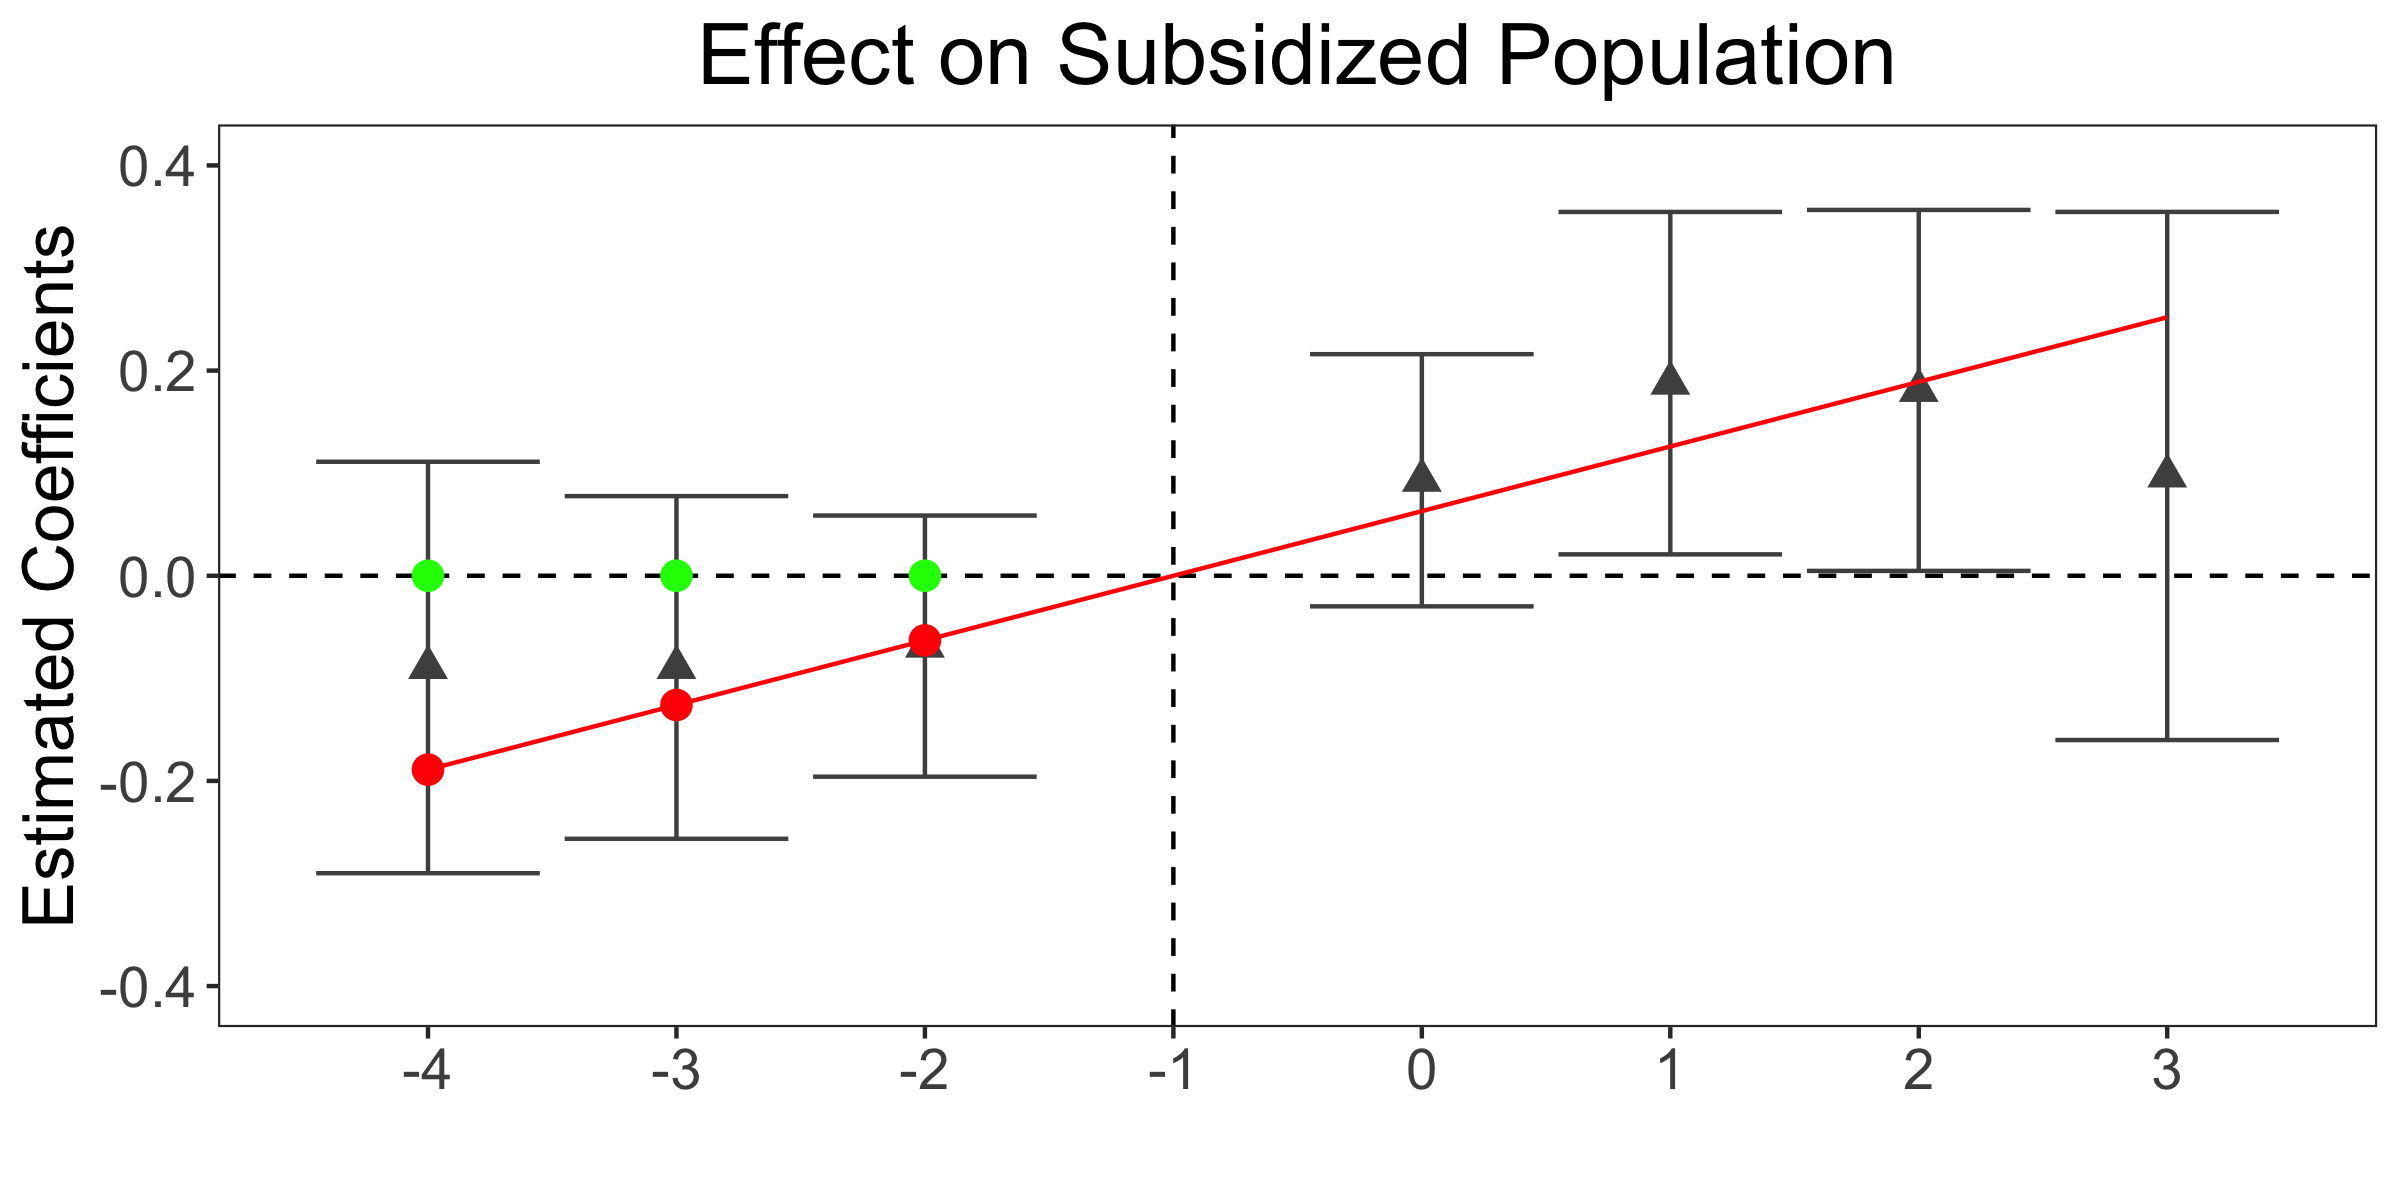
\includegraphics[width = 0.7 \linewidth]{HeAndWang-RedTrend}
	\begin{wideitemize}
		\item
		Are you convinced there's an effect here? Maybe not!
	\end{wideitemize}
\end{onlyenv}


\begin{onlyenv}<+>
	\centering
	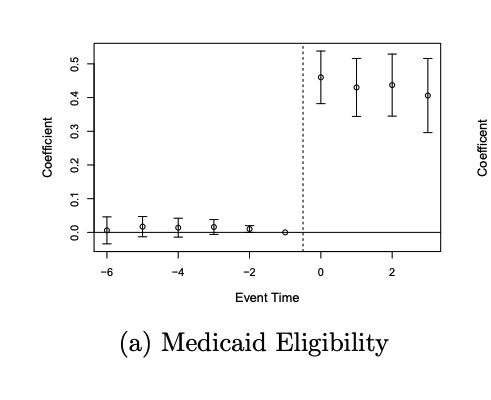
\includegraphics[width = 0.4 \linewidth]{medicaid-eligibility}
	\begin{wideitemize}
		\item
		What about here? 
	\end{wideitemize}
\end{onlyenv}


\begin{onlyenv}<+>
	\centering
	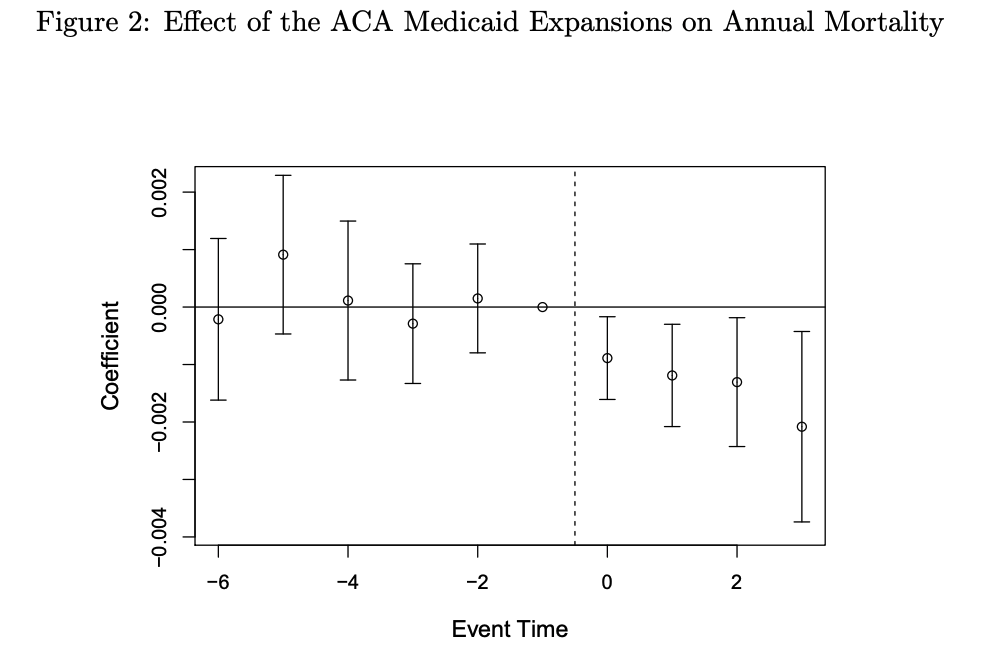
\includegraphics[width = 0.6 \linewidth]{medicaid-mortality}
	\begin{wideitemize}
		\item
		And here?  
	\end{wideitemize}
\end{onlyenv}

\end{frame}

\begin{frame}{Standard Errors for Panel Regressions}
\begin{wideitemize}
	\item
	We know how to get standard errors for OLS estimates of 
	
	$$Y_i = \bm{X}_i'\bm{\beta} + e_i$$
	
	\noindent when $(Y_i,\bm{X}_i)$ are drawn $iid$.
	
	\pause
	\item
	Now, we have 
	
		$$Y_{it} = \bm{X}_{it}'\bm{\beta} + e_{it}$$
		
	\pause
	\item
	Is it reasonable to assume that $(Y_{it}, \bm{X}_{it})$ are $iid$ across $i$ and $t$? \pause{} No
	
	\pause
	\begin{enumerate}
		\item 
		We expect $Y_{i1}$ to be correlated with $Y_{i2}$, e.g., people with high earnings in 2010 also tend to have higher earnings in 2011. This is called \emph{serial autocorrelation} 
		
		\pause
		\item
		More subtlely, if treatment is assigned at the state level, all people in a given state will have the same value of $D_{it}$ (which is included in $\bm{X}_{it}$)
	\end{enumerate}


\end{wideitemize}
\end{frame}

\begin{frame}{Clustered Standard Errors}
	\begin{wideitemize}
		\item 
		\textbf{Clustered standard errors} extend the OLS variance formula to allow $(Y_{it}, \bm{X}_{it})$ to be correlated across observations in the same ``cluster''
		
		\pause
		\item
		The assumption is that each cluster is sampled independently.
		
		\pause
		\item
		For example, if we cluster at the individual level ($i$), then we allow for $Y_{i1}$ and $Y_{i2}$ to be dependent, but assume $(Y_{i1},Y_{i2})$ is independent of $(Y_{j1},Y_{j2})$ for $j\neq i$
		
		\pause
		\item
		In panel analyses, you should at minimum cluster at the individual level to allow for autocorrelation. \pause
		
		\item
		If treatment is assigned at a more aggregate level, it is best to cluster at the level where treatment is assigned.
		
		\pause
		\item
		Keep in mind: the number of ``effective observations'' (used for CLT) is the number of clusters
			\begin{itemize}
				\item 
				Clustered SEs will not be reliable when the number of clusters is very small (e.g. $<20$)
			\end{itemize}	
	\end{wideitemize}
\end{frame}

\begin{frame}{XKCD}
	\centering
	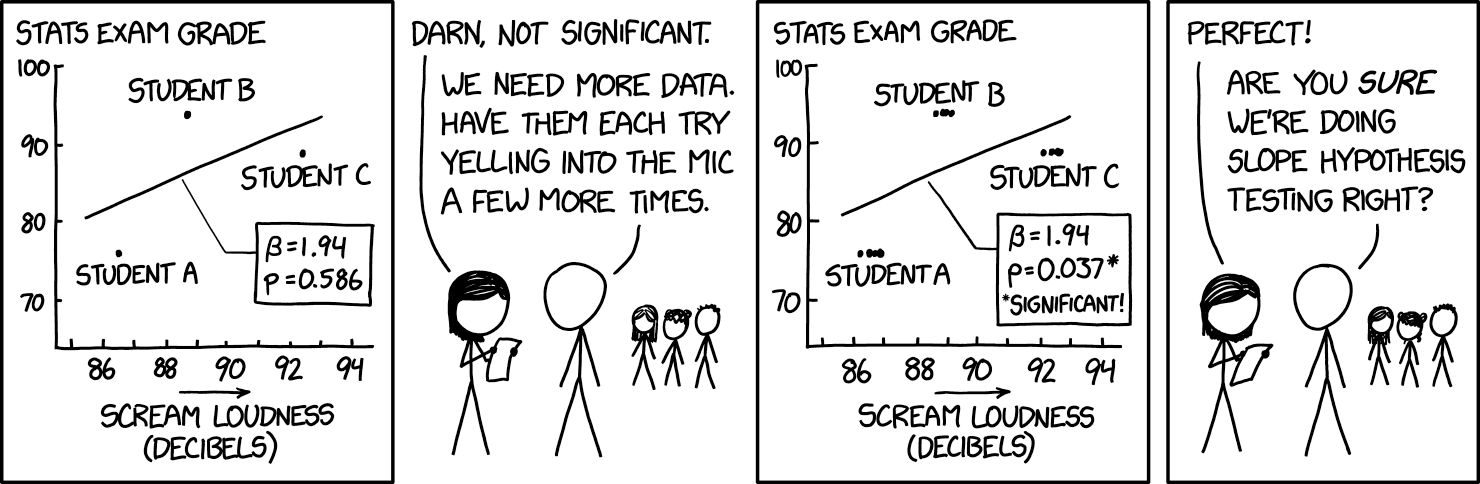
\includegraphics[width=0.9\linewidth]{xkcd}
\end{frame}

\begin{frame}{Implementing Clustered SEs}
	\begin{itemize}
		\item 
		Implementing clustered SEs in Stata is very easy
		
		\item
		Just replace
		
		\begin{quote}
			reg y x, robust
		\end{quote}
	
		\noindent with \\
		
			\begin{quote}
			reg y x, cluster(clustervar)
		\end{quote}
		
	\end{itemize}

\end{frame}

\begin{frame}
		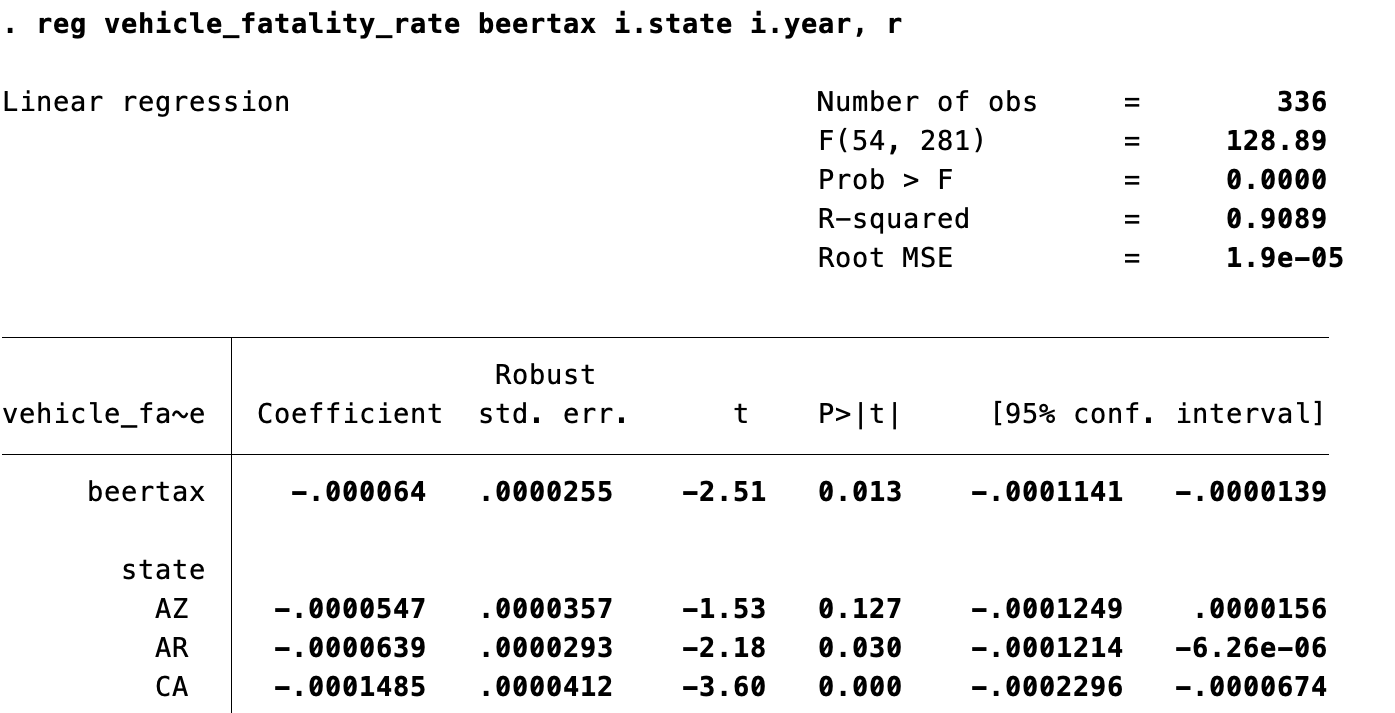
\includegraphics[width = 0.7 \linewidth]{beer-tax1}
	\medskip 
		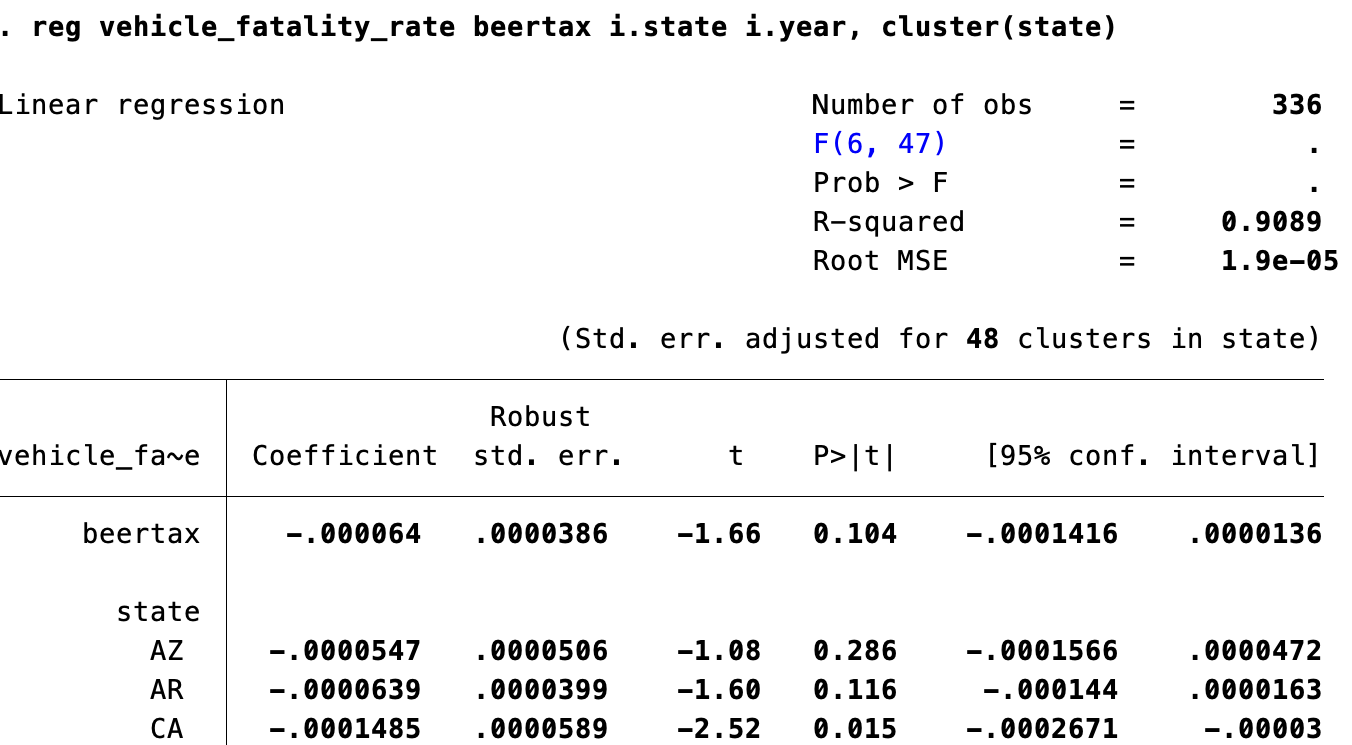
\includegraphics[width = 0.7 \linewidth]{beer-tax2}
	
\end{frame}

\begin{frame}
	\centering
	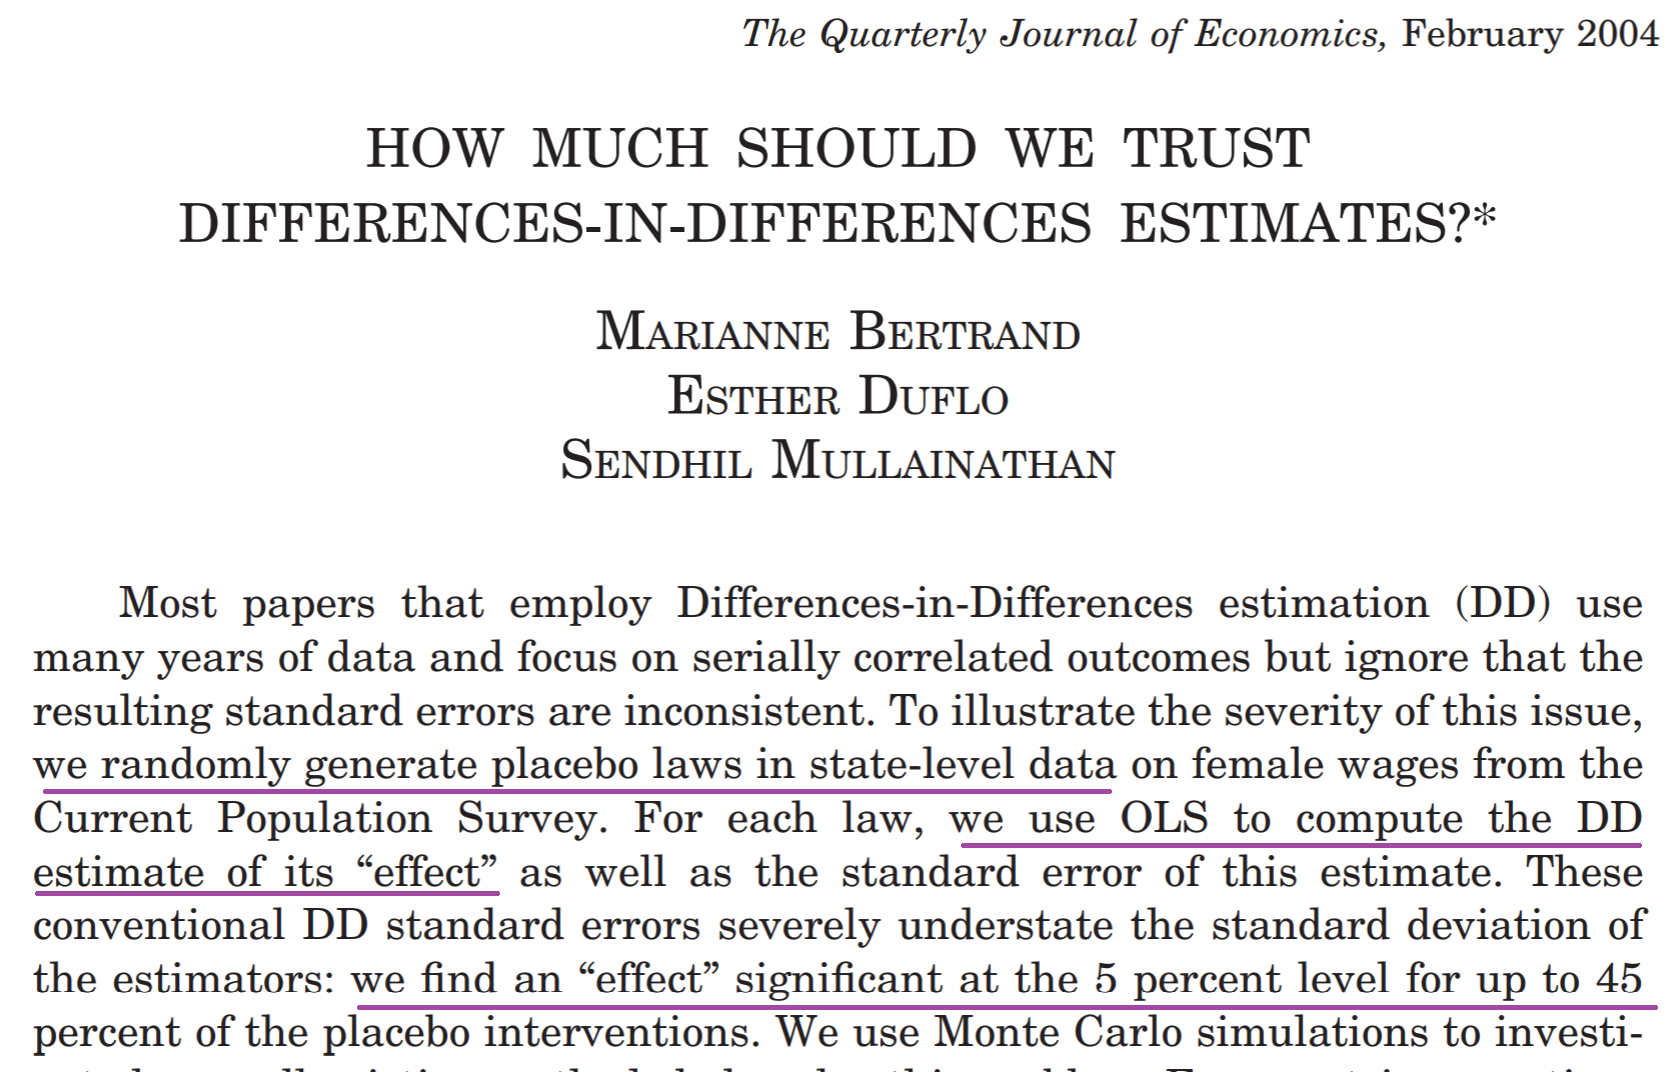
\includegraphics[width = 0.7\linewidth]{bdm04}
\end{frame}


\begin{frame}{A Very Famous DiD}
	\begin{wideitemize}
		\item
		Card and Krueger (1994) ask: how does the minimum wage affect employment? 
		
		\pause
		\item
		How would you expect the MW to affect employment, based on what you learned in micro-economic theory? 
		
		\pause
			\begin{itemize}
				\item 
				In a competitive market, a floor on wages (i.e. the price of labor), should induce a decrease in demand
			\end{itemize}
		
		\pause
		\item
		To study this, CK study an episode in 1992 where NJ raised its minimum wage from \$4.25 to \$5.05
		
		\pause
		\item
		They use a DiD comparing change in employment in fast food restaurants in NJ to that in neighboring PA , where the MW was flat at \$4.25
	\end{wideitemize}
\end{frame}


\begin{frame}
	\begin{center}
			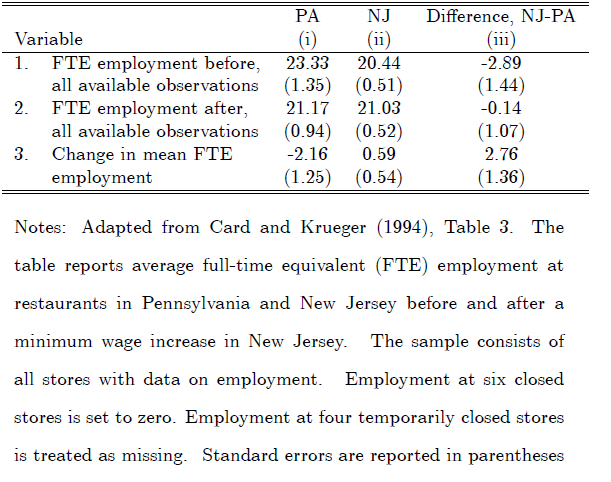
\includegraphics[width = 0.7\linewidth]{CK_table}
	\end{center}
	\pause
	\begin{wideitemize}
		\item
		Point estimates suggest an \textit{increase} in employment of 2.76 FTEs, but not statisticially signfiicant. 
	\end{wideitemize}
\end{frame}

\begin{frame}{Why?!}
	\begin{wideitemize}
		\item
		The result that an increase in the MW does not seem to decrease employment was very surprising (and controversial) at the time
		
		\pause
		\item 
		One explanation for this finding is that labor markets are \textit{not perfectly competitive}. Rather, firms are \textit{monopsonistic}
		
		\pause
		\begin{wideitemize}
			\item
			Consider a firm the employs 100 workers at \$7/hour.
			
			\item
			Suppose hiring another worker would produce an  extra \$10 of profit, but would require raising the wage to \$8/hour.
			
			\pause
			\item
			Should the firm raise the wage to \$8/hour? \pause Not if it means they have to pay all 100 workers an extra \$1!
			
			\pause
			\item
			However, if the MW is raised to \$8/hour, then the firm has to pay the first 100 workers \$8 anyway, and would gladly hire the 101st worker at \$8/hour since this brings \$10 of profit.
		\end{wideitemize}
	\end{wideitemize}
\end{frame}


\begin{frame}
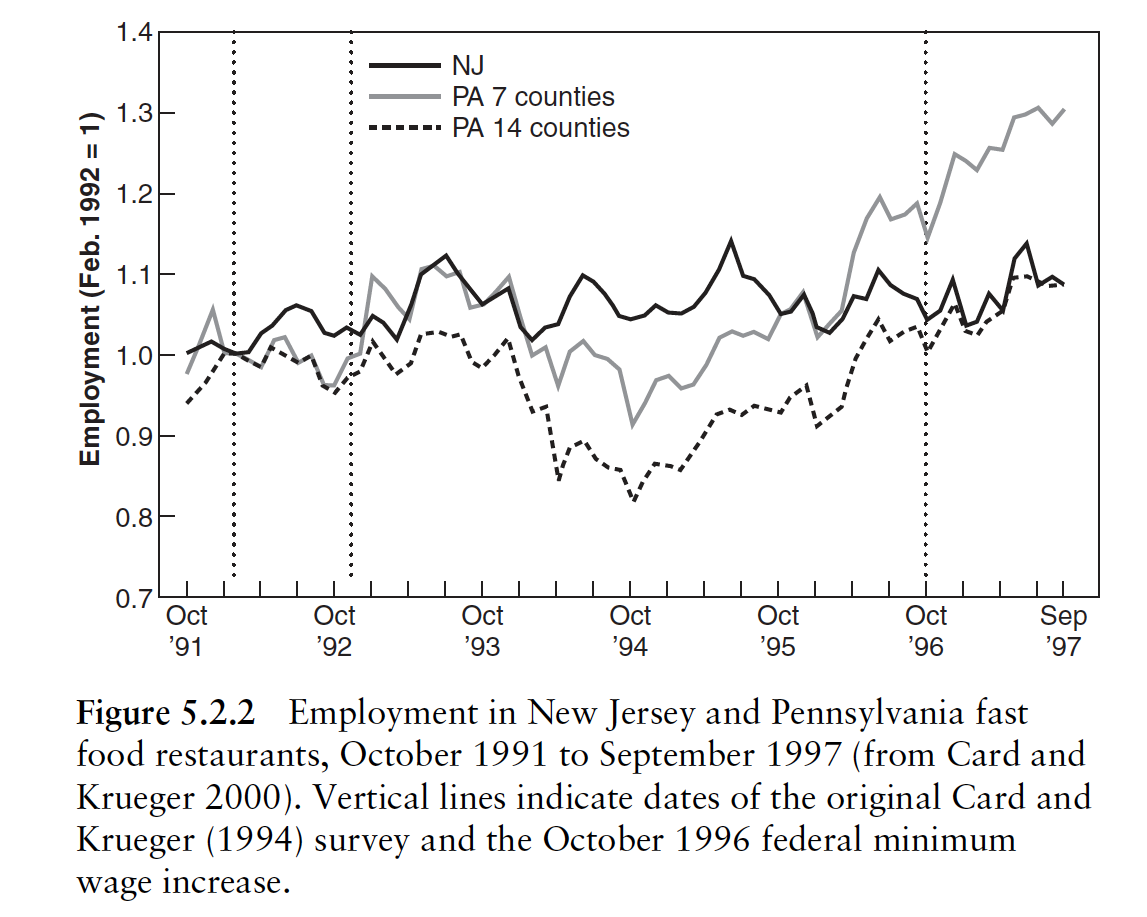
\includegraphics[width = 0.7 \linewidth]{ck_pretrends}	
	
\begin{wideitemize}
	\item
	By modern standards, the CK analysis is perhaps not the most convincing
	
	\pause
	\item
	The two states do not move exactly in parallel even before the policy change in April 1992. \pause
	We also only have 2 states!
\end{wideitemize}
\end{frame}	

\begin{frame}{Staggered Timing}
	\begin{wideitemize}
		\item
		Next I'll show you some more modern evidence on the MW.
		
		\item
		But first we need to discuss DiD when treatment timing is staggered -- e.g., states pass minimum wages in different years 
		
		\pause
		\item
		Until about 5 years ago, people extended DiD to the staggered setting by running OLS regressions like:
		$$Y_{it} = \phi_i + \lambda_t + D_{it} \beta + e_{it}$$
		
		\noindent where $D_{it} = 1$ if unit $i$ is treated in period $t$.
		
		\pause
		\item
		In the two-period model, this corresponds to the diff-in-diff in sample means between treatment and control
		
		\pause
		\item 
		Unfortunately, it turns out that this estimator is \textit{not} an average of DiDs between treated and untreated units in the staggered case.
			\begin{itemize}
				\item 
				See Borusyak and Jaravel (2016), de Chaisemartin and D'Haultfoeuille (2020), Goodman-Bacon (2021)
			\end{itemize}
	\end{wideitemize}
\end{frame}

\begin{frame}
	\begin{wideitemize}
		\item
		Over the last few years, there has been a lot of research about ``fixing'' the issues with these regressions
		
		\item
		The solutions typically involve making ``clean comparisons'' by hand
		
		\pause
		\begin{enumerate}
			\item 
			For units first treated in year $g$, compare outcome change between $g-1$ and $g+k$ to that of units who weren't treated over that period
			
			\pause
			\item
			This is an estimate of the effect $k$ years after treatment for cohort $g$
			
			\pause
			\item
			Do this for every $g$, and then aggregate them to get an average effect
		\end{enumerate}

		\pause
		\item 
		There are many implementations of this and related approaches, including Callaway and Sant'Anna (2020), Sun and Abraham (2020), Borusyak, Jaravel \& Spiess (2021)	
	\end{wideitemize}
\end{frame}

\begin{frame}
	\begin{wideitemize}
		\item
		Cengiz et al (2019) do a modern version of C\&K using 138 MW changes between 1976 and 2016
		
		\pause
		\item
		For each state that changes its MW, they take a ``control group'' of states that didn't change their MW in the 4 years before/after 
		
		\pause
		\item
		They compute a DiD between the treated state and the matched control states
		
		\pause
		\item
		They then take a weighted average of these DiDs to get an overall average effect
	\end{wideitemize}
\end{frame}


\begin{frame}
	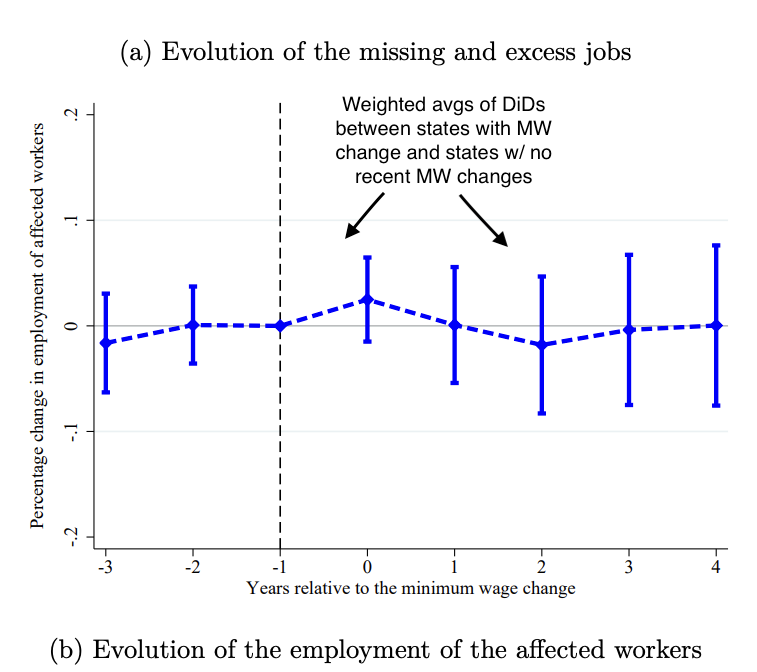
\includegraphics[width =0.9 \linewidth]{cengiz_eventstudy}
\end{frame}


\begin{frame}
	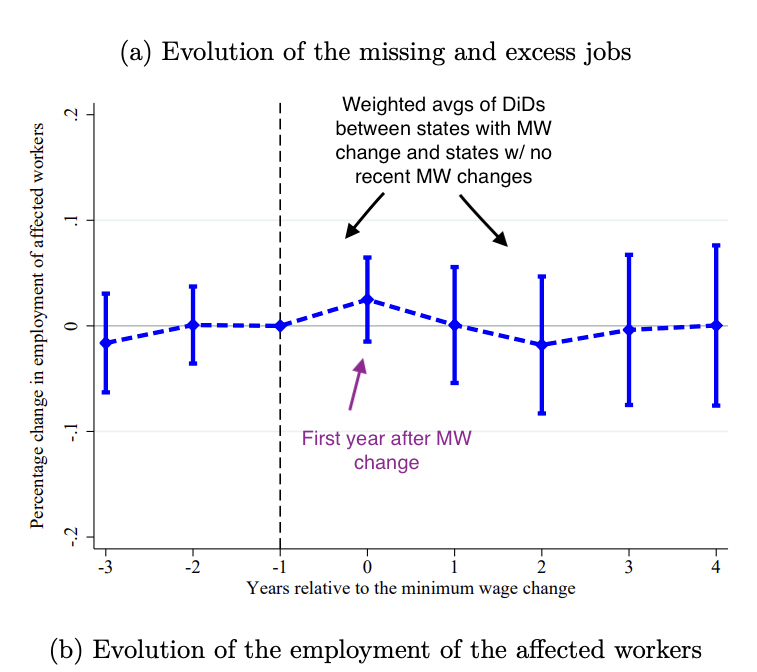
\includegraphics[width =0.9 \linewidth]{cengiz_eventstudy2}
\end{frame}

\begin{frame}
	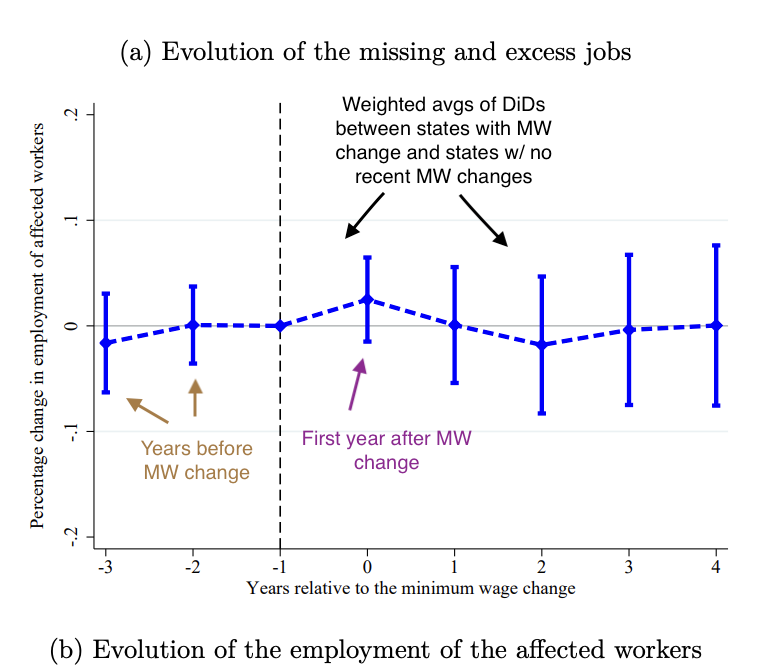
\includegraphics[width =0.9 \linewidth]{cengiz_eventstudy3}
\end{frame}


\begin{frame}{Important Considerations/Caveats}
	\begin{wideitemize}
		\item
		Historical MW changes in the MW have been fairly modest
			\begin{itemize}
				\item 
				Not clear that changes in MW from \$4.25 to \$5.05 are informative abour raises from \$7.25 to \$15!
			\end{itemize}
		
		\pause
		\item
		Historical analyses of MW are typically relatively short-run
			\begin{itemize}
				\item 
				Over long-run, MW increases may induce shifts in technology that replace workers
			\end{itemize}
		
		\pause
		\item
		There is still some debate among economists over whether MWs reduce employment!
	\end{wideitemize}
\end{frame}


\begin{frame}{Other Panel Data Methods}
	\begin{wideitemize}
		\item 
		We've focused on DiD, which is the most commonly-used panel data method in applied micro-economics
		
		\item
		But there are many others:
		
		\begin{itemize}
			\item 
			Controls for lagged dependent variables
			
			\item
			Synthetic control
			
			\item
			Matrix completion
		\end{itemize}
	
		\item
		We won't have time to cover these, but if you're interested, I suggest taking more econometrics classes :) 
	\end{wideitemize}
\end{frame}

%% Clustered SEs


%% Staggered timing

%% Card & Kruger, Dube.




%	Motivation for Panel Data

% Leading intuitive example of DiD

% Introduction to Parallel Trends

% Formal regression analysis of DiD

% Example of regression DiD

% Testing for pretrends

% Examples of good/bad pre-trends

% Something about staggered treatment timing?!

% Card and Krueger; Cengiz 

% Clustering?! 	
	
\end{document}


